%%%%%%%%%%%%%%%%%%%%%%%%%%%%%%%%

% (Replace `SM' with `RB' throughout draft)

%%%%%%%%%%%%%%%%%%%%%%%%%%%%%%%%

% Section 3

2. \textbf{Robot Butler (RB):} 
A simulation of a robot butler in an office building, where the robot's task is 
to navigate between two rooms (of various types) to serve drinks to two people 
(with various roles). This domain has only \~40 permutations of its physical 
object properties and 4 actions in a standard MDP formulation, but has ~1150 
static configurations. Figure~\ref{fig:robotbutler} is a partial illustration 
of one state of the MDP. 

\begin{figure}[t]
  \centerline{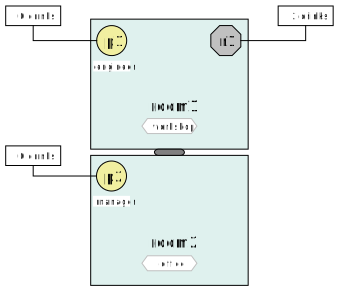
\includegraphics[width=2.5in]{robot-butler-domain}}
  \caption{Example of a scenario in the Robot Butler domain. Depicted is the 
  physical configuration of objects in the domain, as well as static attributes 
  \textit{room type} and \textit{person role}. `p1' and `p2' represent people; 
  the robot is `r1'.}
\label{fig:robotbutler} 
\vspace{1mm}
\end{figure}

%%%%%%%%%%%%%%%%%%%%%%%%%%%%%%%%

% Section 3.1

% Replacing the part beginning ``In the SM domain''

In the RB domain, the fluents are the location of the \textit{robot} and the 
\textit{people} -- we reason about the former and assume the latter are defined 
fluents known at all times. The robot can move between locations, represented 
as an action \textit{move(robot, loc)} and serve a person at a location with 
\textit{serve(robot,person,loc)}. 
We also introduce relations for people's roles, which can be \textit{engineer}, 
\textit{salesperson}, or \textit{manager}, and for rooms, which can be 
\textit{office space}, \textit{conference room}, \textit{kitchen}, or 
\textit{workshop}. Additionally, the scenario has attributes describing whether 
it is early or late in the week and whether people are using equipment. 

%%%%%%%%%%%%%%%%%%%%%%%%%%%%%%%%

% Section 3.1

The RB domain's dynamics are defined using causal laws such as:

\textit{serve(robot,person,loc)} \textbf{causes} \textit{has(person,drink)}

state constraints such as:

\textbf{impossible} \textit{at(person,room2)} \textbf{if} \textit{at(person,room1)}

and executability constraints such as:

\textbf{impossible} \textit{serve(robot,person,loc)} \textbf{if} \textit{has(person,drink)}

%%%%%%%%%%%%%%%%%%%%%%%%%%%%%%%%

% Section 4.2, `Simple Mario'

\subsection{Robot Butler}

In the RB domain,












